\documentclass[tikz]{standalone}
\usepackage{pgfplots}
\pgfplotsset{compat=1.15}
\usepackage{mathrsfs}
\usetikzlibrary{arrows,calc}
\usepackage{tkz-euclide}
\pagestyle{empty}

\definecolor{AngleClr}{rgb}{0,0.39215686274509803,0}
\definecolor{ShapeClr}{rgb}{0.6,0.2,0}
\definecolor{SquareClr}{RGB}{250, 248, 217}
\definecolor{GreenDist}{RGB}{7,122,7}

\begin{document}

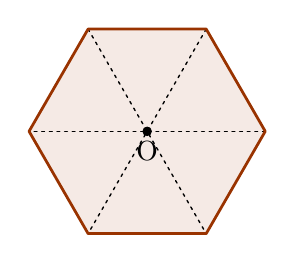
\begin{tikzpicture}[scale=.75]
\tkzSetUpLine[line width=1pt,color=black]
\tkzSetUpPoint[fill=black]

\tkzDefPoints{0/0/O,2/0/P1}
\tkzDefRegPolygon[center,sides=6](O,P1)

\tkzFillPolygon[fill=ShapeClr,fill opacity=0.1](P1,P2,P3,P4,P5,P6)

\tkzDrawSegments[line width=0.5pt,color=black,dashed,dash pattern=on 1pt off 1.75pt](P1,P4 P2,P5 P3,P6)
\tkzDrawPolygon[color=ShapeClr](P1,P2,P3,P4,P5,P6)

\tkzDrawPoints[size=3](O)

\tkzLabelPoint[below](O){$\rm O$}

\end{tikzpicture}
\end{document}
